\newpage
\hypertarget{stringRep vis}{}
\subsection{Implementing stringRep}
\visHeader

\begin{itemize}

\item[$\blacktriangleright$] Visual SDMs support arbitrary nesting of \emph{for each} story nodes via special guards. In \hyperlink{emptyPartition vis}{Section
5.1} we used the \texttt{[end]} edge guard to terminate a loop. Now we'll use a new guard, the \texttt{[each time]}\define{[each time]} guard, to indicate control flow that is \emph{nested} and
executed for each match. Go ahead and create the SDM for \texttt{Box::toString} until it closely resembles Fig.~\ref{fig:sdm_tostring_1}. 

\vspace{0.5cm}

\begin{figure}[htbp]
\begin{center}
  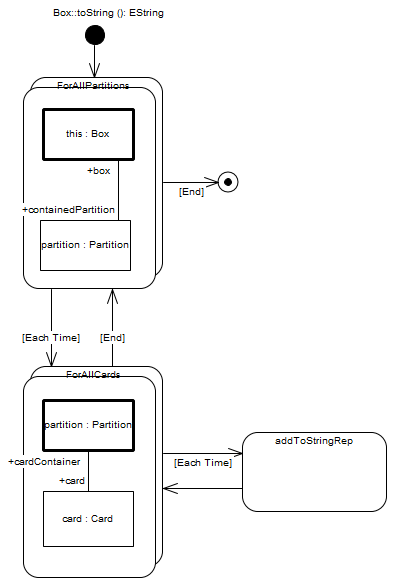
\includegraphics[width=0.8\textwidth]{ea_toStringStart}
  \caption{Control flow with nested loops} 
  \label{fig:sdm_tostring_1}
\end{center}
\end{figure}

\clearpage

\item[$\blacktriangleright$] Now, while the \texttt{addToStringRep} activity node has been created, its default type will not allow it to invoke our helper
method. Double-click the node to invoke its properties dialogue and change its \texttt{type} to a \texttt{StatementNode}(Fig.~\ref{fig:updateStatement}). 

\vspace{0.5cm}

\item[$\blacktriangleright$] Before closing, switch to the \texttt{Statement} tab (Fig.~\ref{fig:editStatement}) to construct a \texttt{MethodCallExpression}.
We want to access the \texttt{Box} object (\texttt{this}) and its \texttt{addToStringRep} method. Update the \texttt{Parameter Values} to \texttt{card} so we
can pass the object variable \texttt{card} to the method as parameter. Although \texttt{card} can just be entered, the best practice is to double-click the
field to pop-up a new dialogue. This way complex expressions can be constructed by repeatedly double-clicking the fields.

\vspace{0.5cm}

\begin{figure}[htbp]
   \centering
      \subfloat[Update the \texttt{addToStringRep} node]{
        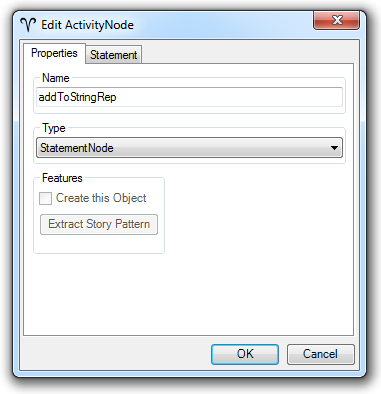
\includegraphics[width=0.5\textwidth]{ea_updateToStatement}
        \label{fig:updateStatement}
      }
      \subfloat[Edit the \texttt{MethodCallExpression} ]{
        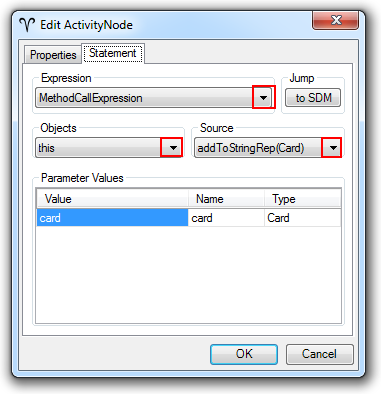
\includegraphics[width=0.5\textwidth]{ea_editStatementNode}
        \label{fig:editStatement}
      }
      \caption{}
\end{figure}
\FloatBarrier

\end{itemize}

Statement nodes can be used to interact with methods that are implemented by hand as they provide a means of invoking libraries and arbitrary Java code from
SDMs. Please note that we do not differentiate at this point between methods that are implemented via an SDM or by hand and thus, statement nodes can of course
be used to invoke other SDMs via a MethodCallExpression. Most importantly, this enables \emph{recursion} as the current SDM can be invoked on \texttt{this} with
appropriate new arguments.

\newpage

\begin{itemize}

\item[$\blacktriangleright$] To complete the SDM, return the final string representation value of the box via an \texttt{AttributeValueExpression} in
the stop node (Fig.~\ref{fig:toStringStopNode}).\define{AttributeValue\-Expression}This is a new expression type we haven't encountered before. Its name is
fairly self-explanatory however, as all it does it update and bind the return \texttt{stringRep} attribute to the value edited in each instance of
\texttt{addToStringRep}. How is this expression similar to a \texttt{Parameter\-Expression}?

\vspace{0.5cm}

\begin{figure}[htbp]
\begin{center}
  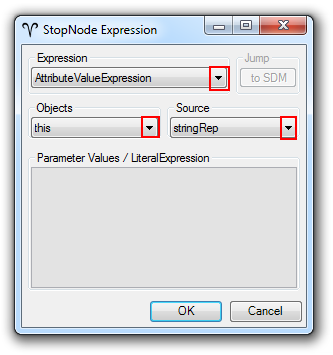
\includegraphics[width=0.5\textwidth]{ea_returnAttributeStopNode}
  \caption{Specify a return value}
  \label{fig:toStringStopNode}
\end{center}
\end{figure}

\vspace{0.5cm}

\item[$\blacktriangleright$] Take some time to compare and reflect on the complete SDM as depicted in Fig.~\ref{fig:sdm_tostring_5}.  The idea was to abstract
from the actual text representation of the box and model the necessary traversal of the data structure. The helper method \texttt{addToStringRep} could, for
example, build up a string buffer and update this string representation. While modelling this SDM, we have seen that \emph{for each} story nodes can be nested,
and have learnt two new uses of \emph{MethodCallExpressions} that provide a type safe means of invoking methods from SDMs.

\vspace{0.5cm}

\item[$\blacktriangleright$] As always, save, validate, and build your metamodel in Eclipse. To see how this is done in the
textual syntax, check out the nested loops in Fig.~\ref{fig:toStringFlow} and each pattern in Fig.~\ref{fig:toStringPatterns}.

\newpage

\vspace*{2cm}

\begin{figure}[htbp]
\begin{center}
  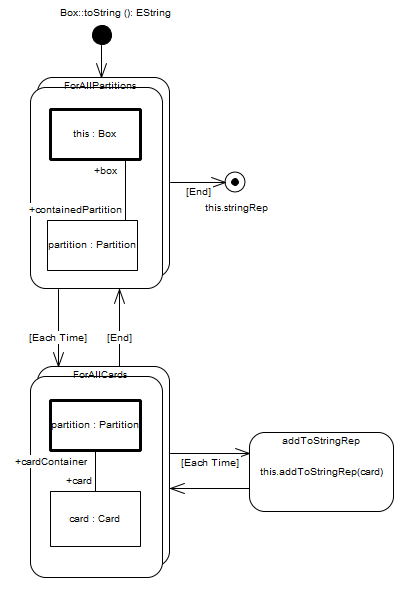
\includegraphics[width=0.8\textwidth]{ea_toStringComplete}
  \caption{The complete SDM for \texttt{Box::toString}}  
  \label{fig:sdm_tostring_5}
\end{center}
\end{figure}
\FloatBarrier

\jumpSingle{sec:fastCard}

\end{itemize}
